This chapter contains the implementation of the protocol designed in Chapter \ref{cha:protocolDesign}. 

First, the classes used in the implementation are shown and explained. Then important parts of the code are explained.
 

\section{General}
The implementation is written in C++.

\section{Classes}
The solution contains two different running applications. The main node and the sensor nodes. There are two sets of code due to the different requirements of the nodes. For example, the main node does not have a sensor, so it should not be able to handle a sensor.

This section contains the differences in the applications, and the classes contained in each application.

\subsubsection*{Main node}
The main node is a Raspberry Pi device, running the Raspbian operating system. The classes in the main node application is seen on Figure \ref{fig:mainnodeClass}.
The main node pairs nodes and handles receiving data.

\begin{figure}[h!]
\centering
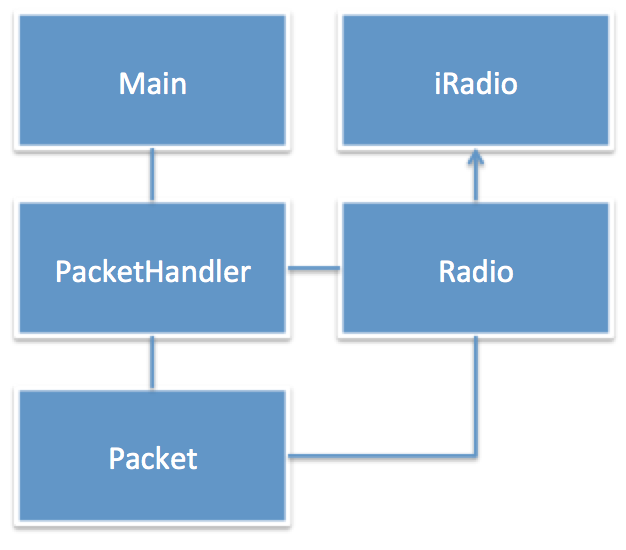
\includegraphics[width=0.8\textwidth]{chapters/implementation/figures/mainnodeClass.png}
\caption{Classes used in the main node.}
\label{fig:mainnodeClass}
\end{figure}



\subsubsection*{Sensor nodes}
The platform on the nodes are comprised of Arduino Uno or Mega. The difference in the two platforms are the pins used with the sensors and radio modules. Besides that, the code on the platforms are the same.

The classes used in the nodes are seen on Figure \ref{fig:nodeClass}.
\begin{figure}[h!]
\centering
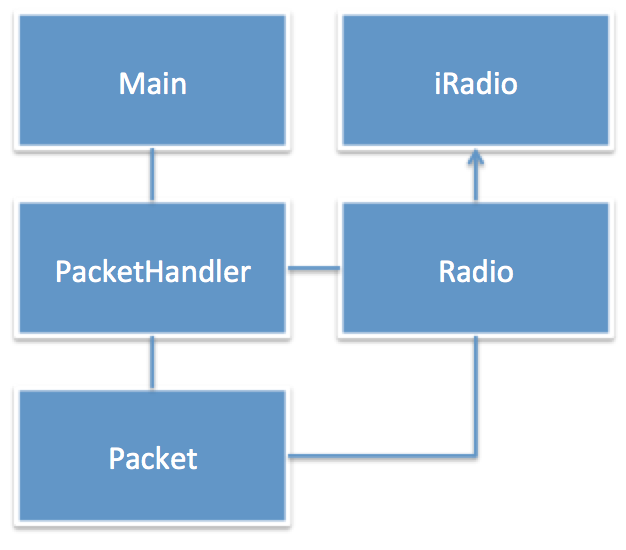
\includegraphics[width=0.75\textwidth]{chapters/implementation/figures/nodeClass.png}
\caption{Classes used in nodes.}
\label{fig:nodeClass}
\end{figure}


\subsubsection*{Class descriptions}
This section contains explanations about the classes used in the nodes.

\begin{description}
\item[Main] \hfill \\
The \textit{Main} class is the entrypoint in the application. This class initializes the components, and a \textit{PacketHandler} object.

Contains one or more \textit{Sensor}s, a \textit{Radio} object, and a \textit{PacketHandler} object. The sensors and radio objects are passed along to the \textit{PacketHandler} on instantiation.

\item[iRadio and iSensor] \hfill \\
The \textit{iSensor} and \textit{iRadio} interfaces are used to create a certain way that all sensors and radio module classes should work. This means that replacing or adding a new sensor or using another radio module is not a problem, as the rest of the application knows that the radio is able to send and receive, and the sensor is able to return a value. 
It is not necessary to know how it is done, only that it is possible. These interfaces are used to set a standard on how to communicate with them, whether it is a moisture sensor or a pH sensor.

Every type of radio or sensor added to the node will inherit from these interfaces.


\textit{iSensor} only contains the method \textit{double read()}, that returns the value of the sensor. \todo{Kan være der er mere?}

\textit{iRadio} contains a method for sending a packet, \textit{void send(Packet packet)}. \todo{Kan være der er mere?}

\item[Sensor] \hfill \\
The \textit{Sensor} class can be used for multiple sensors, as long as the sensor class inherits from \textit{iSensor}. This class' job is to read data from a sensor on the node, handle this data, and return it to the class that requested this data.

In the solution, as the moisture sensor is used, the sensor class is called \textit{MoistureSensor}. This class can only be found on the sensor nodes, and not on the main node.


\item[Radio] \hfill \\
The \textit{Radio} class handles the radio communication. Types of this class should inherit from the \textit{iRadio} interface. The \textit{Radio} class notifies the \textit{PacketHandler} when a packet is received. It is also able to send packets given from other classes.

\item[PacketHandler] \hfill \\
The \textit{PacketHandler} handles all packets received. This class is a singleton, as only one is needed in the application. This class is instantiated from the entrypoint.

\textit{PacketHandler} receives a call from the \textit{Radio} object when a packet is received, passing a \textit{Packet} object created from the packet. The \textit{PacketHandler} then determines wether or not to act on this packet. 
For example, should a node receive a pair request, this should be ignored, as only the main node acts on such requests. The same thing happens on the main node. Should the main node receive a data request, this will of course be ignored.
If a response to the node is required, the \textit{PacketHandler} will manage this process. This could be getting a reading from the sensor and sending it back, or relaying data from another node to the parent.

\item[Packet] \hfill \\
The class \textit{Packet} contains the ability to parse a packet from a string to a \textit{Packet} object, along with the properties required to further handle the packet. This includes the type, and possibly sensor values, from/to values or an identifier from the main node.

This class is passed between the \textit{Radio} and \textit{PacketHandler}, when sending and receiving packets.

\end{description}


\section{Code?}